\section{3D Coordinate Systems}

\subsection{3D Space}
Similar to the 2D coordinate system, we have the $x$ and $y$-axes. In addition, we add a new vertical $z$-axis. The direction of $z$-axis is determined by the right-hand rule. Such system is called the right-hand system.

\begin{figure}[h]
    \centering
    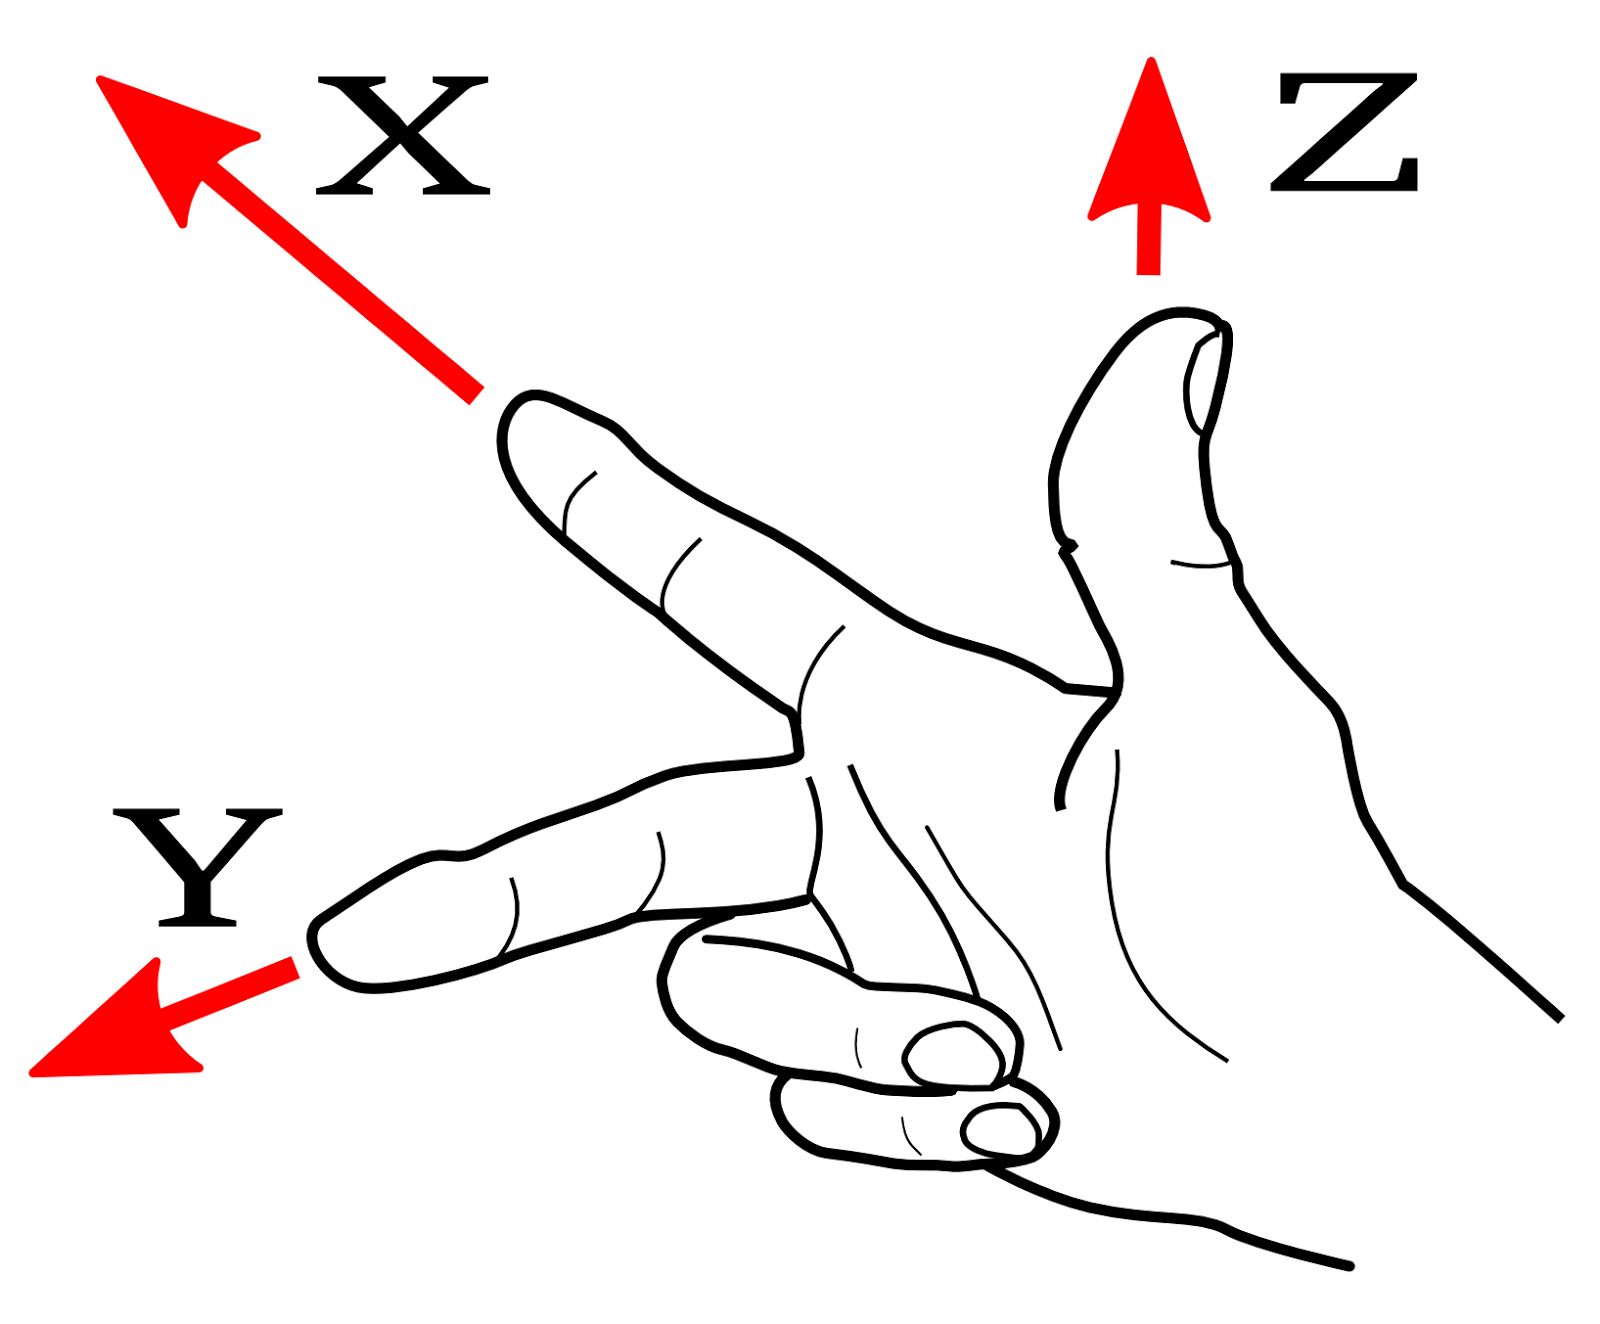
\includegraphics[width=0.3\textwidth]{figures/right-hand-rule.png}
    \caption{Right-hand rule}
\end{figure}
\hfill

In a right-hand system, the axes $x,y,z$ goes in clockwise, following ``index finger, middle finger, thumb''. The thumb pointing up is the $z$-axis. The origin $O$ is located at $(0,0,0)$.

Each two of the three axes form planes, giving us three planes: $xy,xz,yz$-planes.

We can project a point in the 3D coordinate onto the planes. For the point $P=(a,b,c)$, its projection onto $xy$-plane is $(a,b,0)$. Similarly, its projection onto $yz,xz$-planes are $(0,b,c)$ and $(a,0,c)$, respectively.

The Cartesian product $\R\times\R\times\R = \{(x,y,z) \mid x,y,z\in\R\}$ is the set of ordered triples of real numbers. It is denoted $\R^3$. These triples correspond to points in the three-dimensional coordinate.

\subsection{Surfaces and Solids}
Geometrically, equations involving $x,y,z$ represents a surface in $\R^3$. A 2D line is analogous to a plane in 3D, and a 2D circle is analogous to a cylinder in 3D.

\begin{example}
What surface in $\R^3$ is represented by each of the following equations? \\ (a) $z-3$ (b) $y-5$

(a) The equation $z-3$ represents the set $\{(x, y, z) \mid z - 3\}$, which is the set of all points in $\R^3$ whose z-coordinate is 3 ($x$ and $y$ can each be any value). This is the horizontal plane that is parallel to the $xy$-plane and three units above it.

(b) The equation $y-5$ represents the set of all points in $\R^3$ whose $y$-coordinate is 5. This is the vertical plane that is parallel to the $xz$-plane and five units to the right of it.
\end{example}

\subsection{Distance Formula}

The distance formula is similar to the distance formula in 2D.

\begin{theorem}[Distance formula in 3D]
The distance $|P_1P_2|$ between points $P_1=(x_1,y_1,z_1)$ and $P_2=(x_2,y_2,z_2)$.
$$
|P_1P_2| = \sqrt{(x_2-x_1)^2+(y_2-y_1)^2+(z_2-z_1)^2}
$$
\end{theorem}

The set of points that are equidistant to a point forms a sphere shell in 3D.

\begin{theorem}[Equation of sphere]
An equation of a sphere with center $C=(h,k,l)$ and radius $r$ is
$$
(x-h)^2+(y-k)^2+(z-l)^2 = r^2
$$
In particular, if the center is the origin, then an equation of the sphere is
$$
x^2+y^2+z^2 = r^2
$$
\end{theorem}

\section{Vectors}

\subsection{Definition}

Formally, we define vectors in the following way:

\begin{definition}[Vector Space]
A vector space is a field $(V,+,\cdot)$ where $V$ is a set of objects called vectors, together with a rule $+:\, V\times V\to V$ for adding $\alpha,\beta\in V$ to product $\alpha+\beta\in V$ and another rule $\cdot:\, V\times V\to V$ for multiplying vector $v\in V$ by any $k\in\R$ to produce $kv\in V$. In addition, the field must satisfy that

\begin{multicols}{2}
\begin{enumerate}
    \item $\alpha+\beta = \beta+\alpha$
    \item $(\alpha+\beta)+\gamma = \alpha+(\beta+\gamma)$
    \item $\alpha+0=\alpha$
    \item $\alpha+(-\alpha)=0$
    \item $k(\alpha+\beta)=k\alpha+k\beta$
    \item $(k+s)\alpha=k\alpha+s\alpha$
    \item $k(s\alpha)=(ks)\alpha$
    \item $1\alpha=\alpha$
\end{enumerate}
\end{multicols}
for the zero vector $0$, $s,k\in\R$, and $-\alpha \in V$ for all $\alpha \in V$.
\end{definition}

Given the appropriate, many things can be vector, including polynomials, matrices, etc. However, conventionally, when we say ``vector'', we refer to directed line segments in $\R^n$, where the zero vector is simply a line segment with length zero. This is the type of vectors that is commonly used in physics.

The way we add vectors is by connecting them tip to tail. This is called the Triangle Law or Parallelogram Law.

\begin{figure}[h]
    \centering
    \includesvg{figures/vector-addition.svg}
    \caption{Triangle Law}
\end{figure}

The difference of two vectors is simply defined as
$$
\vv{u}-\vv{v} = \vv{u}+(-\vv{v})
$$
We can write vectors in terms of coordinates, and the coordinates are called the components of the vector.

Given the points $A=(x_1,y_1,z_1)$ and $B=(x_2,y_2,z_2)$, the vector (directed line segment) from $A$ to $B$, denoted $\vv{AB}$ can be obtained by subtracting the coordinates of $A$ from $B$.
$$
\vv{AB}=(x_2-x_1,y_2-y_1,z_2-z_2)
$$

\begin{definition}[Norm]
The norm or magnitude of a vector $\vv{v}=(x,y,z)$ is
$$
\norm{\vv{a}} = \sqrt{x^2+y^2+z^2}
$$
\end{definition}

\begin{definition}[Unit vectors]
Vectors whose norm is 1 is called the unit vectors. In particular,
$$
\vv{i}=(1,0,0) \qquad \vv{j}=(0,1,0) \qquad \vv{k}=(0,0,1)
$$
are called the standard basis vectors.
\end{definition}

\begin{theorem}
Every vector in $V_3$ (the set of vectors in 3D) can be expressed as a linear combination of $\vv{i},\vv{j},\vv{k}$.

\begin{proof}
\hfill \\
Let $a=(x,y,z) \in V_3$ be arbitrary. Then, we can write
\begin{align*}
    \vv{a} &= (x,y,z) \\
    &= (x,0,0)+(0,y,0)+(0,0,z) \\
    &= x(1,0,0)+y(0,1,0)=z(0,0,1) \\
    &= x\vv{i} + y\vv{j} + z\vv{k}
\end{align*}
\end{proof}
\end{theorem}

\subsection{Properties}

\begin{theorem}[Cauchy-Schwartz Inequality]
For vectors $\vv A, \vv B$,
$$
|A\cdot B| \leq \norm{A}\norm{B}
$$
The equality only holds when $A$ and $B$ are parallel.

\begin{proof}
    \hfill \\
    Let $A$ and $B$ be arbitrary vectors.
    Define $P(t)=\norm{A}-2t(A\cdot B)+\norm{B}^2t^2 = (\norm{A-tB})^2$
    
    $P(t)$ will always be non-negative. Then, $P(t)=0$ has one or no solution.
    
    This implies that the discriminant $\Delta \leq 0$.
    
    By definition of the discriminant
    \begin{align*}
        \Delta = (-2(A \cdot B))^2 -4 \norm{B}^2 \norm{A}^2 &\leq 0 \\
        4(A\cdot B)^2 &\leq 4 \norm{A}^2\norm{B}^2 \\
        \sqrt{(A\cdot B)^2} & \leq \sqrt{\norm{A}^2\norm{B}^2}
    \end{align*}
    We can take out the square root. Hence, $|A\cdot B| \leq \norm{A}\norm{B}$.
    
    By generalization, for all vectors, the Cauchy-Schwartz Inequality holds.
\end{proof}
\end{theorem}

\begin{theorem}[Triangle Inequality]
For vectors $\vv A, \vv B$,
$$
\norm{\vv u + \vv v} \leq \norm{\vv u} + \norm{\vv v}
$$

\begin{proof}
    \hfill \\
    Let $\vv u$ and $\vv v$ be arbitrary.
        
    By property of vector arithmetic,
    \begin{align*}
        \norm{\vv u + \vv v}^2 &= (\vv u + \vv v)\cdot (\vv u + \vv v) \\
        &= \vv u \cdot \vv v + 2\vv u \cdot \vv v + \vv v \cdot \vv v \\
        &= \norm{\vv u}^2 + 2(\vv u \cdot \vv v) + \norm{\vv v}^2
    \end{align*}

    By property of absolute value,
    $$
    \norm{\vv u}^2 + 2(\vv u \cdot \vv v) + \norm{\vv v}^2 \leq \norm{\vv u}^2 + 2 |\vv u \cdot \vv v| + \norm{\vv v}^2
    $$
    By Cauchy-Schwartz Inequality
    $$
    \norm{\vv u}^2 + 2 |\vv u \cdot \vv v| + \norm{\vv v}^2 \leq \norm{\vv u}^2 + 2 \norm{\vv u}\norm{\vv v} + \norm{\vv v}^2
    $$
    Then,
    $$
    \norm{\vv u + \vv v}^2 \leq (\norm{\vv u}+\norm{\vv v})
    $$
    Taking square root of both side gives
    $$
    \norm{\vv u + \vv v} \leq \norm{\vv u} + \norm{\vv v}
    $$
    By generalization, for all vectors $\vv u$ and $\vv v$, the Triangle Inequality holds.
\end{proof}
\end{theorem}


\section{The Dot Product}
\subsection{Definition and Properties}

\begin{definition}[The Dot Product]
The dot product between vectors $A=(x_1,y_1,z_1)$ and $B=(x_2,y_2,z_2)$ is defined as
$$
A \cdot B = x_1x_2+y_1y_2+z_1z_2
$$
\end{definition}

The dot product has the following properties:
\begin{multicols}{2}
\begin{enumerate}
    \item $\vv a \cdot \vv a = \norm{\vv a}^2$
    \item $\vv a \cdot \vv b = \vv b \cdot \vv a$
    \item $\vv a \cdot (\vv b+\vv c) = \vv a\cdot \vv b+ \vv a \cdot \vv c$
    \item $(c\vv a)\cdot \vv b= c(\vv a\cdot \vv b)=\vv a\cdot(c\vv b)$
    \item $\vv 0 \cdot \vv a = \vv 0$
\end{enumerate}
\end{multicols}

\begin{theorem}
If $\theta$ is the angle between $\vv a$ and $\vv b$,
$$
\vv a \cdot \vv b = \norm{\vv a}\norm{\vv b}\cos\theta
$$

\begin{proof}
\hfill \\
By the Law of Cosines,
$$
\norm{\vv a -\vv b}^2 = \norm{\vv a}^2 + \norm{\vv b}^2  - 2\norm{\vv a}\norm{\vv b}\cos\theta
$$
Also,
\begin{align*}
    \norm{\vv a-\vv b}^2 &= (\vv a - \vv b)\cdot (\vv a - \vv b) \\
    &= \norm{\vv a}^2 - 2\vv a \cdot \vv b + \norm{\vv b}^2
\end{align*}
Substitute this back to the first equation,
\begin{align*}
    \norm{\vv a}^2 - 2\vv a \cdot \vv b + \norm{\vv b}^2 &= \norm{\vv a}^2 + \norm{\vv b}^2  - 2\norm{\vv a}\norm{\vv b}\cos\theta \\
    - 2\vv a \cdot \vv b &= - 2\norm{\vv a}\norm{\vv b}\cos\theta \\
    \vv a \cdot \vv b &= \norm{\vv a}\norm{\vv b}\cos\theta
\end{align*}
\end{proof}
\end{theorem}

\begin{corollary}\label{cos-dot-product}
If $\theta$ is the angle between nonzero vectors $\vv a$ and $\vv b$
$$
\cos\theta = \frac{\vv a \cdot \vv b}{\norm{\vv a}\norm{\vv b}}
$$
\end{corollary}

If the dot product between two vectors is positive, then the angle $\theta$ between two vectors is acute, $0\degree \leq \theta < 90\degree$; if the dot product is negative, $90\degree < \theta \leq 180\degree$; if the dot product equals zero, $\theta = 90\degree$.

\subsection{Direction Angles and Directional Cosines}

\begin{definition}[Direction Cosines]
For a non-zero vector $\vv a = (a_1,a_2,a_3)$, let $\alpha,\beta,\gamma$ be the angles that $\vv a$ makes with the $x,y,z$-axes. From Corollary \ref{cos-dot-product},
$$
\cos\alpha = \frac{\vv a \vv i}{\norm{\vv a}\norm{\vv i}} = \frac{a_1}{\norm{\vv a}} \qquad \cos\beta = \frac{\vv a \vv j}{\norm{\vv a}\norm{\vv j}} = \frac{a_2}{\norm{\vv a}} \qquad \cos\gamma = \frac{\vv a \vv k}{\norm{\vv a}\norm{\vv k}} = \frac{a_3}{\norm{\vv a}}
$$
Those values are called the direction cosines.
\end{definition}

It follows that
$$
\frac{\vv a}{\norm{\vv a}} = (\cos\alpha,\cos\beta,\cos\gamma)
$$

\subsection{Projection and Component}

\begin{definition}
\hfill \\
Scalar projection of $\vv b$ onto $\vv a$:
$$
\comp_a b = \frac{\vv a \cdot \vv b}{\norm{\vv a}}
$$
Vector projection of $\vv b$ onto $\vv a$:
$$
\proj_a b = \left(\frac{\vv a \cdot \vv b}{\norm{\vv a}}\right)\frac{\vv a}{\norm{\vv a}} = \frac{\vv a \cdot \vv b}{\norm{\vv a}^2}\vv{a}
$$
\end{definition}

The derivation of the vector projection is as follows:

\begin{proof}
\hfill \\
Since $\proj_{B}{A}$ is the projection of $\vv A$ onto $\vv B$, $\proj_{B}{A}$ is parallel to $\vv B$. It implies that there exists some $k \in \R$ such that $\proj_B{A}=k{\vv B}$.

Also, there exists some vector $\vv\alpha$ such that $\vv A + \vv a = \proj_B A$ and $\vv\alpha \cdot \vv B = 0$, that is $\vv\alpha$ is orthogonal to $\vv B$. On the picture below, $\vv\alpha$ is the red vector.

\begin{figure}[h]
    \centering
    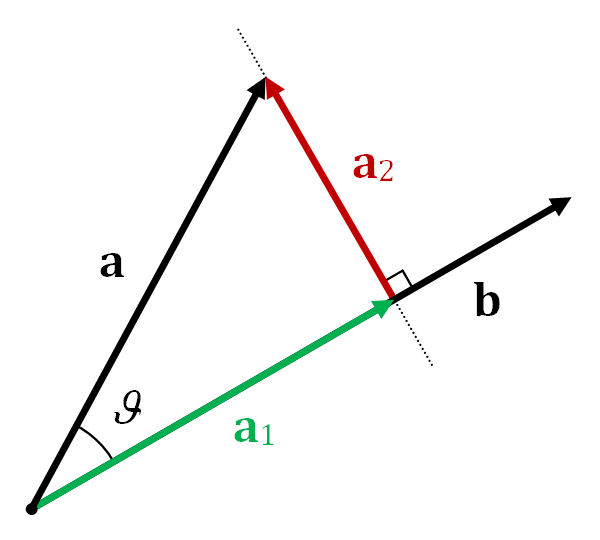
\includegraphics[width=0.3\linewidth]{figures/projection.png}
    \caption{Vector projection}
    \label{fig:projection}
\end{figure}

From that, we have the following equation:
\begin{align*}
    \vv B \cdot (\vv A + \vv \alpha) &= \vv B \cdot \proj_B A \\
    \vv B \cdot (\vv A + \vv \alpha) &= \vv B \cdot (k \vv B) \\
    \vv B \cdot (\vv A + \vv \alpha) &= k (\vv B \cdot \vv B) \\
    \vv B \cdot \vv A + \vv B \cdot \vv \alpha &= \vv B \cdot (k \vv B) \\
    \vv B \cdot \vv A &= \vv B \cdot (k \vv B) & \text{since $\vv\alpha \cdot \vv B = 0$} \\
    k &= \frac{\vv A \cdot \vv B}{\vv B \cdot \vv B}
\end{align*}

Hence,
$$
\proj_B A = \left( \frac{\vv A \cdot \vv B}{\vv B \cdot \vv B} \right) \vv B
$$
In addition, $\comp_B A$ is the norm of $\proj_B A$.
\end{proof}

\section{The Cross Product}
\subsection{Definition}

Recall that the dot product between $A=(x_1,y_1,z_1)$ and $B=(x_2,y_2,z_2)$ is defined as
$$
A \cdot B = x_1x_2+y_1y_2+z_1z_2
$$
but also
$$
A \cdot B = \norm{A}\norm{B}\cos\theta
$$
where $\theta$ is the angle between $A$ and $B$.

The dot product gives us a scalar. We will now define the cross product, which gives us a vector. The cross product $\vv a \times \vv b$ is a vector that is orthogonal to both $\vv a$ and $\vv b$.

\begin{figure}[ht]
    \centering
    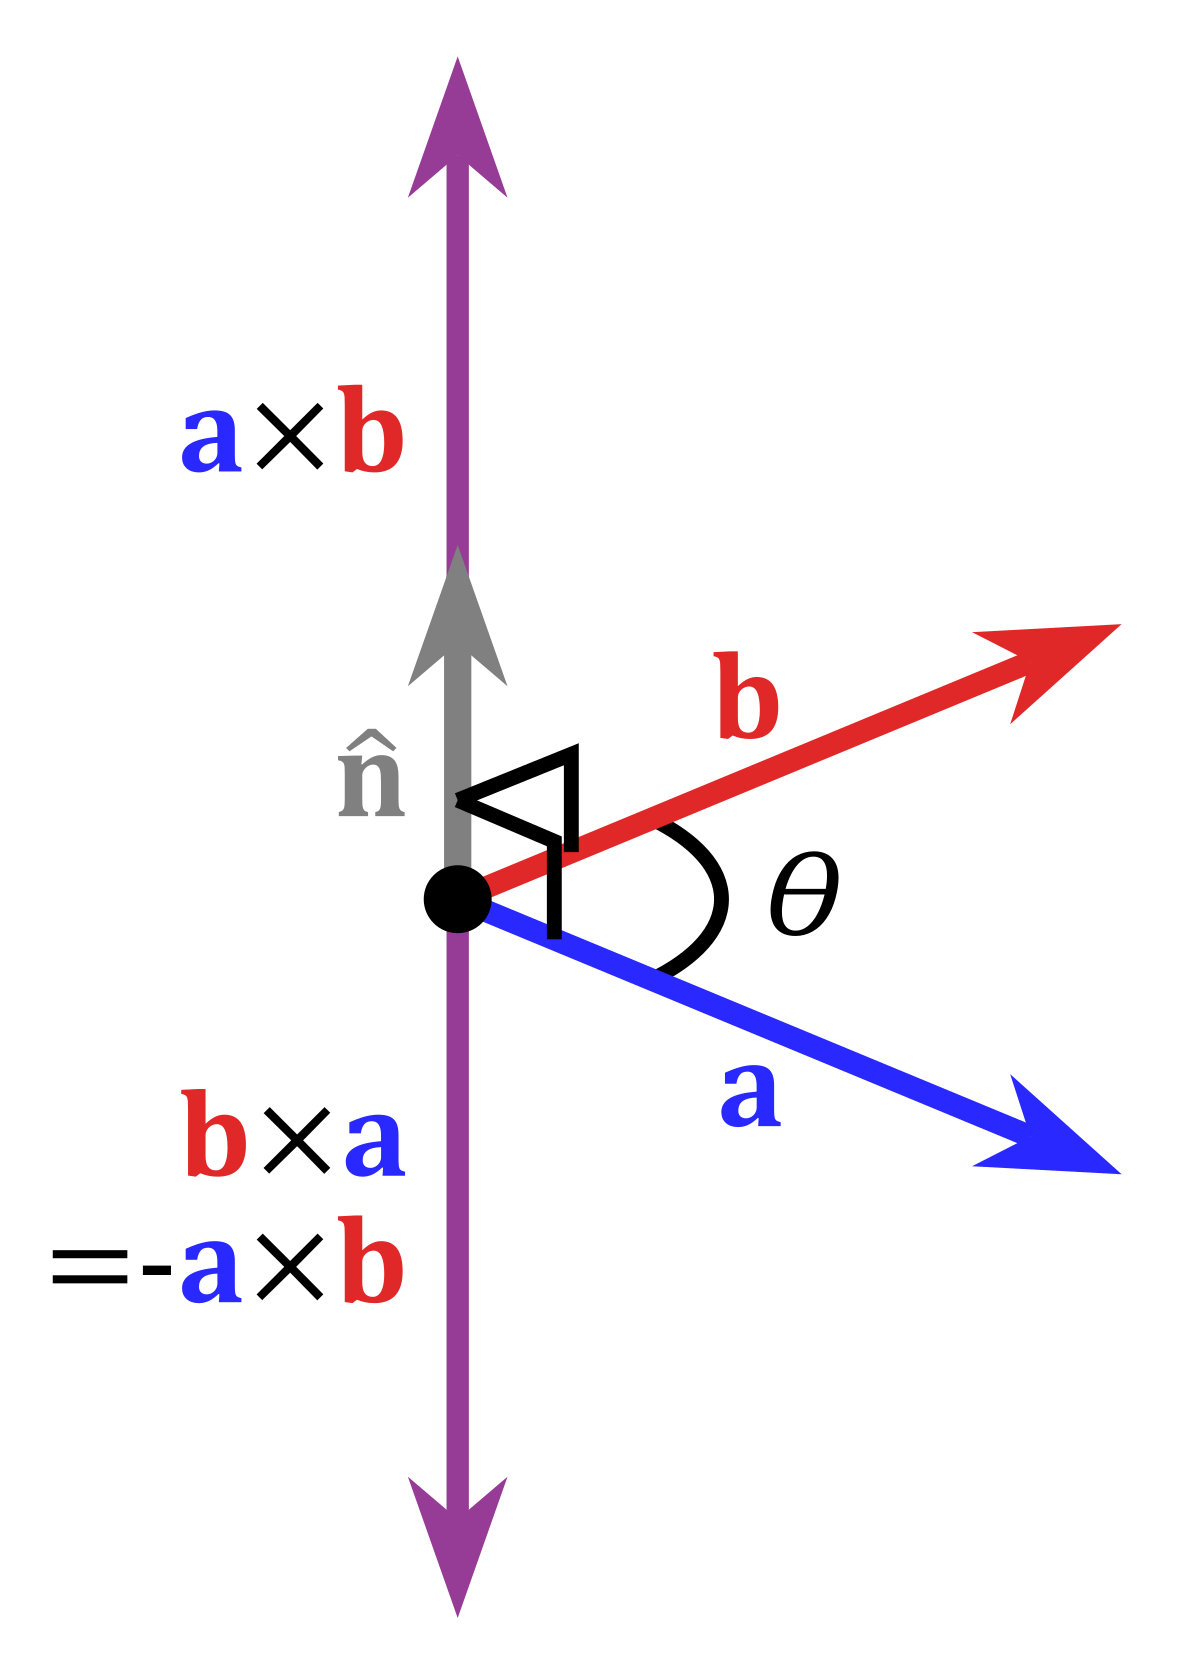
\includegraphics[width=0.3\linewidth]{figures/cross-product.png}
    \caption{The Cross Product}
\end{figure}

Importantly, the cross product is not commutative, i.e. in general, $\vv a \times \vv b \neq \vv b \times \vv a$.

\begin{definition}[The Dot Product]
For vectors $A = (a_1,b_1,c_1)$ and $B=(b_1,b_2,b_3)$ in $\R^3$, 
\begin{align*}
    A \times B &= \begin{vmatrix}
    \vv i & \vv j & \vv k \\
    a_1 & a_2 & a_3 \\
    b_1 & b_2 & b_3
    \end{vmatrix} = \vv i \begin{vmatrix}
    a_2 & a_3 \\
    b_2 & b_3
    \end{vmatrix} - \vv j \begin{vmatrix}
    a_1 & a_3 \\
    b_1 & b_3
    \end{vmatrix} + \vv k \begin{vmatrix}
    a_1 & a_2 \\
    b_1 & b_2
    \end{vmatrix} \\
    &= (a_2b_3-b_2a_3,\, b_1a_3-a_1b_3,\, a_1b_2-b_1a_2)
\end{align*}
\end{definition}

\begin{theorem}
$$
\vv a \times \vv b = \norm{\vv a}\norm{\vv b}\sin\theta
$$
Hence, if $\theta=0$, $\norm{\vv a \times \vv b} = 0$; if $\theta=90$, then $\norm{\vv a \times \vv b}=\norm{\vv a}\norm{\vv b}$; if $\theta=180$, $\norm{\vv a \times \vv b} = 0$.
\end{theorem}

\begin{theorem}[Area of Parallelogram]
The parallelogram defined by the vectors $\vv a, \vv b$ is the norm of their cross product.
$$
A = \norm{\vv a}(\norm{\vv b}\sin\theta) = \norm{\vv a \times \vv b}
$$
\end{theorem}

\subsection{Triple Product}

\begin{definition}
The triple product $\vv a \cdot (\vv b \times \vv c)$ is defined as
$$
\vv a \cdot (\vv b \times \vv c) = \begin{vmatrix}
a_1 & a_2 & a_3 \\
b_1 & b_2 & b_3 \\
c_1 & c_2 & c_3
\end{vmatrix} = (\vv a \times \vv b) \cdot \vv c
$$
\end{definition}

\begin{theorem}
The volume of the parallelepiped determined by vectors $\vv a,\vv b,\vv c$ is the magnitude of the triple product.
$$
V=Ah=\norm{\vv b \times \vv c}\norm{\vv a}|\cos\theta|=\norm{\vv a \cdot (\vv b \times \vv c)}
$$
\end{theorem}

\subsection{Properties}

\begin{multicols}{2}
\begin{enumerate}
    \item $\vv a \times \vv b = - \vv b \times \vv a$
    \item $(c\vv a) \times \vv b = c(\vv a \times \vv b) = \vv a \times (c \vv b)$
    \item $\vv a \times (\vv b + \vv c) = \vv a \times \vv b + \vv a \times \vv c$
    \item $(\vv a + \vv b) \times \vv c = \vv a \times \vv c + \vv b \times \vv c$
    \item $\vv a \cdot (\vv b \times \vv c) = (\vv a \times \vv b) \cdot \vv c$
    \item $\vv a \times (\vv b \times \vv c) = (\vv a \cdot \vv c)\vv b - (\vv a \cdot \vv b)\vv c$
\end{enumerate}
\end{multicols}